% ===========================================
\subsection{A convenient way to visualize numerical semigroups}\label{subsec:visualization-and-figures}
The pictures in this paper were produced using the \textsf{GAP}~\cite{GAP4-2018} package \textsf{IntPic}~\cite{IntPic-2017}, while the computations have been carried out using the \textsf{GAP} package \textsf{numericalsgps}~\cite{Numericalsgps-2018}.

Let $S$ be a numerical semigroup. The set of nonnegative integers up to $\conductoroper+\multiplicityoper-1$ clearly contains $\leftsoper$ and it is easy to see that it contains $\primitivesoper$ as well. It is helpful to dispose the mentioned integers into a table and to highlight those that, in some sense, are special.

Several figures will be presented to give pictorial views of numerical semigroups. Each of them consists of a rectangular $(\qoper+1)\times \multiplicityoper$-table and the entries corresponding to elements of the semigroup are highlighted in some way. Some gaps can also be emphasized. The entries in uppermost row are those of the threshold interval. 

\begin{example}\label{ex:gens-5-13_cond-20}
	Figure~\ref{fig:gens-5-13_cond-20} is a pictorial representation of the numerical semigroup $\langle 5,13 \rangle_{20}=\langle 5,13,21,22,24 \rangle$. 
	%$\langle 5,13 \rangle_{20}$. 
	The elements of the semigroup are highlighted and, among them, the primitive elements and the conductor are emphasized. When an element is highlighted for more than one reason, gradient colours are used. 
	%This semigroup is of maximal embedding dimension.
	
\thisfloatsetup{floatwidth=.35\hsize,capbesidewidth=sidefil,capposition=beside,capbesideposition=right}
%\thisfloatsetup[figure]{floatwidth=.35\hsize}
	\begin{figure}[h]
		\begin{center}
			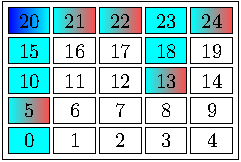
\includegraphics[scale=0.8]{gens-5-13_cond-20.pdf}
		\end{center}
		\caption{Pictorial representation of the numerical semigroup $\langle 5,13,21,22,24 \rangle$. \label{fig:gens-5-13_cond-20}}
	\end{figure} 
\end{example}

Observe that there is at most one primitive per column. There is exactly one in each column when the semigroup is  of maximal embedding dimension. 

Note that all the integers in a given column are congruent modulo $\multiplicityoper$. In particular, an element belongs to the Apéry set relative to $\multiplicityoper$ if and only if it is the lowest emphasized element %(i.e., that belongs to $S$) 
in some column (provided that no gaps (for instance the pseudo-Frobenius numbers) are highlighted). 
\medskip

For the benefit of the reader, I explain the way I produced Figure~\ref{fig:gens-5-13_cond-20}, including the \textsf{GAP} code used. 
To start, \textsf{GAP} is taught what my numerical semigroup is (see the manual of \textsf{numericalsgps} for details).
\begin{verbatim}
	ns := NumericalSemigroup(5,13,21,22,24);
\end{verbatim}
Then one can use the following commands to produce the \textsf{TikZ} code for the picture shown (which can be included in a \LaTeX\ document):
\begin{code}\label{code:draw}
\begin{verbatim}
	#cls is given just to make a change to the default colors
	cls := [ "blue","-red","red!70", "black!40" ];
	P := MinimalGenerators(ns);
	m := Multiplicity(ns);
	c := Conductor(ns);
	q := CeilingOfRational(c/m);
	rho := q*m-c;
	list := [-rho .. c+m-1];
	ti := [c..c+m-1]; 
	importants := Union(SmallElements(ns),ti);
	options := rec(colors := cls,highlights:=[[c],importants,P]);
	tkz := IP_TikzArrayOfIntegers(list,m,options);;	
	Print(tkz);
\end{verbatim}
\end{code}
The function \texttt{IP\_TikzArrayOfIntegers} (which produces the \textsf{TikZ} code from the information previously computed using \textsf{numericalsgps}) is part of the \textsf{intpic} package. The manual of the package can be consulted for details and examples. In particular, the manual contains a complete example showing a possible way to include the picture (or its \textsf{TikZ} code) in a \LaTeX\ document.

Executing the following command, the created picture should pop up. As this command depends on some other software, namely the operating system, some extra work on the configuration may be needed.
\begin{verbatim}
IP_Splash(tkz);
\end{verbatim}
If everything goes well, the figure (in \textsf{pdf} format) can be saved and included in the \LaTeX\ document in some standard way.
\begin{example}\label{ex:sgp-with-PF}
	Figure~\ref{fig:sgp-with-PF} is just another example. The following \textsf{GAP} session shows some important data: a numerical semigroup and its pseudo-Frobenius numbers. These are highlighted in the figure, in addition to elements of the semigroup, as in Example~\ref{ex:gens-5-13_cond-20}.
	\begin{verbatim}
	gap> ns := NumericalSemigroup(12, 19, 20, 22, 23, 26, 27, 28, 29);;
	gap> Conductor(ns);
	38
	gap> pf := PseudoFrobenius(ns);
	[ 16, 30, 33, 37 ]	
	\end{verbatim}
	
\thisfloatsetup{floatwidth=.41\hsize,capbesidewidth=sidefil,capposition=beside,capbesideposition=right}
%\thisfloatsetup[figure]{floatwidth=.35\hsize}
	\begin{figure}[h]
		\begin{center}
			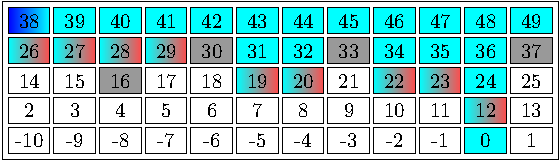
\includegraphics[scale=0.8]{sgp-with-PF.pdf}
		\end{center}
		\caption{Pictorial representation of %the numerical semigroup 
			$\langle 12, 19, 20, 22, 23, 26, 27, 28, 29 \rangle$, with the pseudo-Frobenius numbers highlighted. \label{fig:sgp-with-PF}}
	\end{figure} 
\end{example}

The picture can be obtained with just small changes from \textsf{GAP}-code~\ref{code:draw}.
Besides redefining the numerical semigroup, it suffices to replace the line beginning with \textsf{options} by the following two lines of code:
    
\begin{verbatim}
	pf := PseudoFrobenius(ns);;
	options := rec(colors := cls,highlights:=[[c],importants,P,pf]);;
\end{verbatim}

In order to obtain an image just showing the shape, the options can be changed as follows:
\begin{code}\label{code:shape}
\begin{verbatim}# options to produce the shape
	options := rec(
	highlights:=[[],[],[c],importants,[],[],[],[],P],
	cell_width := "6",colsep:="0",rowsep:="0",inner_sep:="2",
	shape_only:=" ",line_width:="0",line_color:="black!20");;	
\end{verbatim}
\end{code}	

\thisfloatsetup{floatwidth=.43\hsize,capbesidewidth=sidefil,capposition=beside,capbesideposition=right}
%\thisfloatsetup[figure]{floatwidth=.35\hsize}
\begin{figure}[h]
	\begin{center}
		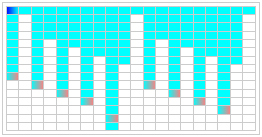
\includegraphics[scale=1.8]{GAS_m20_h2_d9_l8.pdf}
	\end{center}
	\centering
	\caption{Shape of the semigroup $\langle 20, 49, 58, 67, 76, 85, 94, 103, 112\rangle$ }\label{fig:GAS_m20_h4_d9_l6}
%gap> m := 20;; h := 2;; d := 9;; l := 8;;
%gap> gens := List([1..l], k -> h*m + k*d);
%[ 49, 58, 67, 76, 85, 94, 103, 112 ]
%gap> ns := NumericalSemigroup(Union([m],gens));
%<Numerical semigroup with 9 generators>
%gap> draw_for_W0_shape(ns);	
\end{figure}

% ===========================================
 
